\documentclass{article}

\usepackage[utf8]{inputenc}
\usepackage[top=2cm, left=2cm, right=2cm, bottom=2cm]{geometry}
\usepackage{subfig}
\usepackage{graphicx}

\title{Homework 6 - Clustering \\
        \vspace{5px} \large UTFPR - CPGEI - Data Mining \\
        Prof. Dr. Heitor Silvério Lopes}
\author{Vinícius Couto Tasso}
\date{October, 2019}

\begin{document}

\maketitle

\section*{Physiotherapy dataset}


\indent The physiotherapy dataset contains information gathered from 300 different patients of a physiotherapy clinic. Each patient has 6 attributes representing some kind of physical condition. It is known that in the dataset there is a group of healthy patients and a group of patients that suffer from some kind of skeletal muscle condition.

Since there is no information about the number of medical conditions present on the dataset or even the meaning of collected data, methods of clustering were applied to help identify different groups of patients inside the dataset.


The ideal number of clusters to be identified by the algorithm was found empirically, repeating the experiment with values for $k$ ranging from 2 to 8. The Silhouette Scores for each clustering task showed that the best result was obtained for 2 clusters, supposedly healthy and non-healthy patients.

The results showed that \textit{V6}, the last feature of the dataset, was the one to provide better separability for $k = 2$.

\begin{figure}[htbp]
\centering
    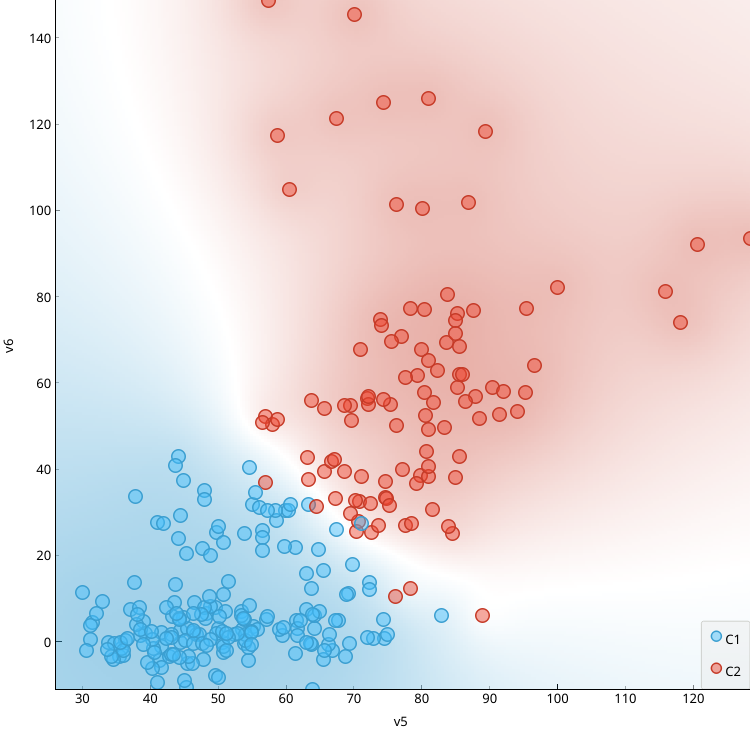
\includegraphics[scale=0.5]{v5vsv6.png}
    \caption{Scatter plot of data that offers the best separability in 2 different clusters.}
    \label{fig:kmeans_scatter_plot}%
\end{figure}

It is easy to note that, on Figure \ref{fig:kmeans_scatter_plot} representation, the C1 cluster is much more densely packed and tight together than the C2 cluster. Besides, it is the cluster with most samples, with almost twice as much data (194 vs 106). It is assumed that the dataset is richer in samples of healthy patients and that healthy patients are more similar to one another than non-healthy patients, due to the possibility of the latter being affected by different medical conditions. Therefore, we assume that the C1 cluster represents the healthy people of the dataset.

\begin{figure}[htbp]
    \centering
        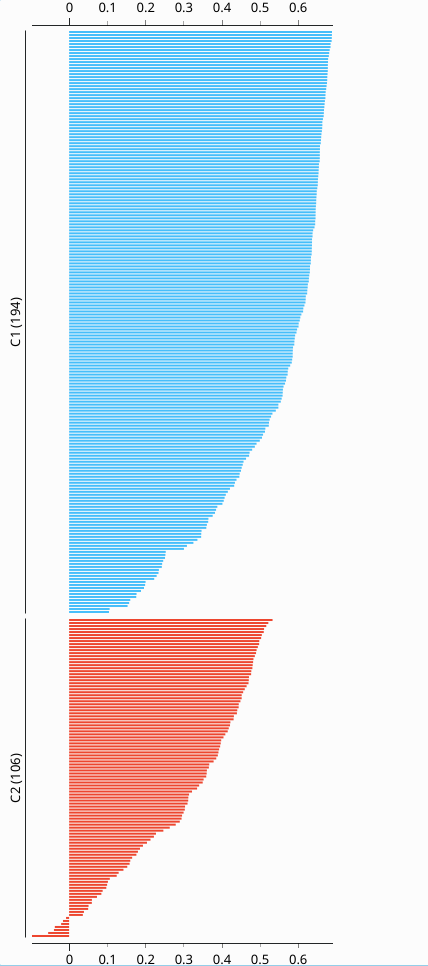
\includegraphics[height=10cm]{euclidean_silhouette.png}
    \caption{Silhouette Score of the k-Means output calculated using euclidean distances.}
    \label{fig:silhouette_score}
\end{figure}

The Silhouette Score shown in Figure \ref{fig:silhouette_score} confirms that C1 is indeed much more well-behaved, but also shows that, in both clusters, there is a significant amount of data that is not well represented. This is a strong indicative that there may be several clusters that the k-Means approach could not identify. For instance, C2 could be divided into ``Medical Condition A'' and ``Medical Condition B'', resulting in a total of 3 clusters. 

The hierarchical clustering was performed to compare the obtained results. For the task of hierarchical clustering, Euclidean distances and Ward linkage were used.  The results, shown in Figure \ref{fig:hierarchical}, are similar to those obtained in the previous experiment. This clustering result confirms that C1 and C2 are very well defined and separated, but shows how many lesser clusters can be formed from the previous ones.

\begin{figure}[htbp]
    \centering
    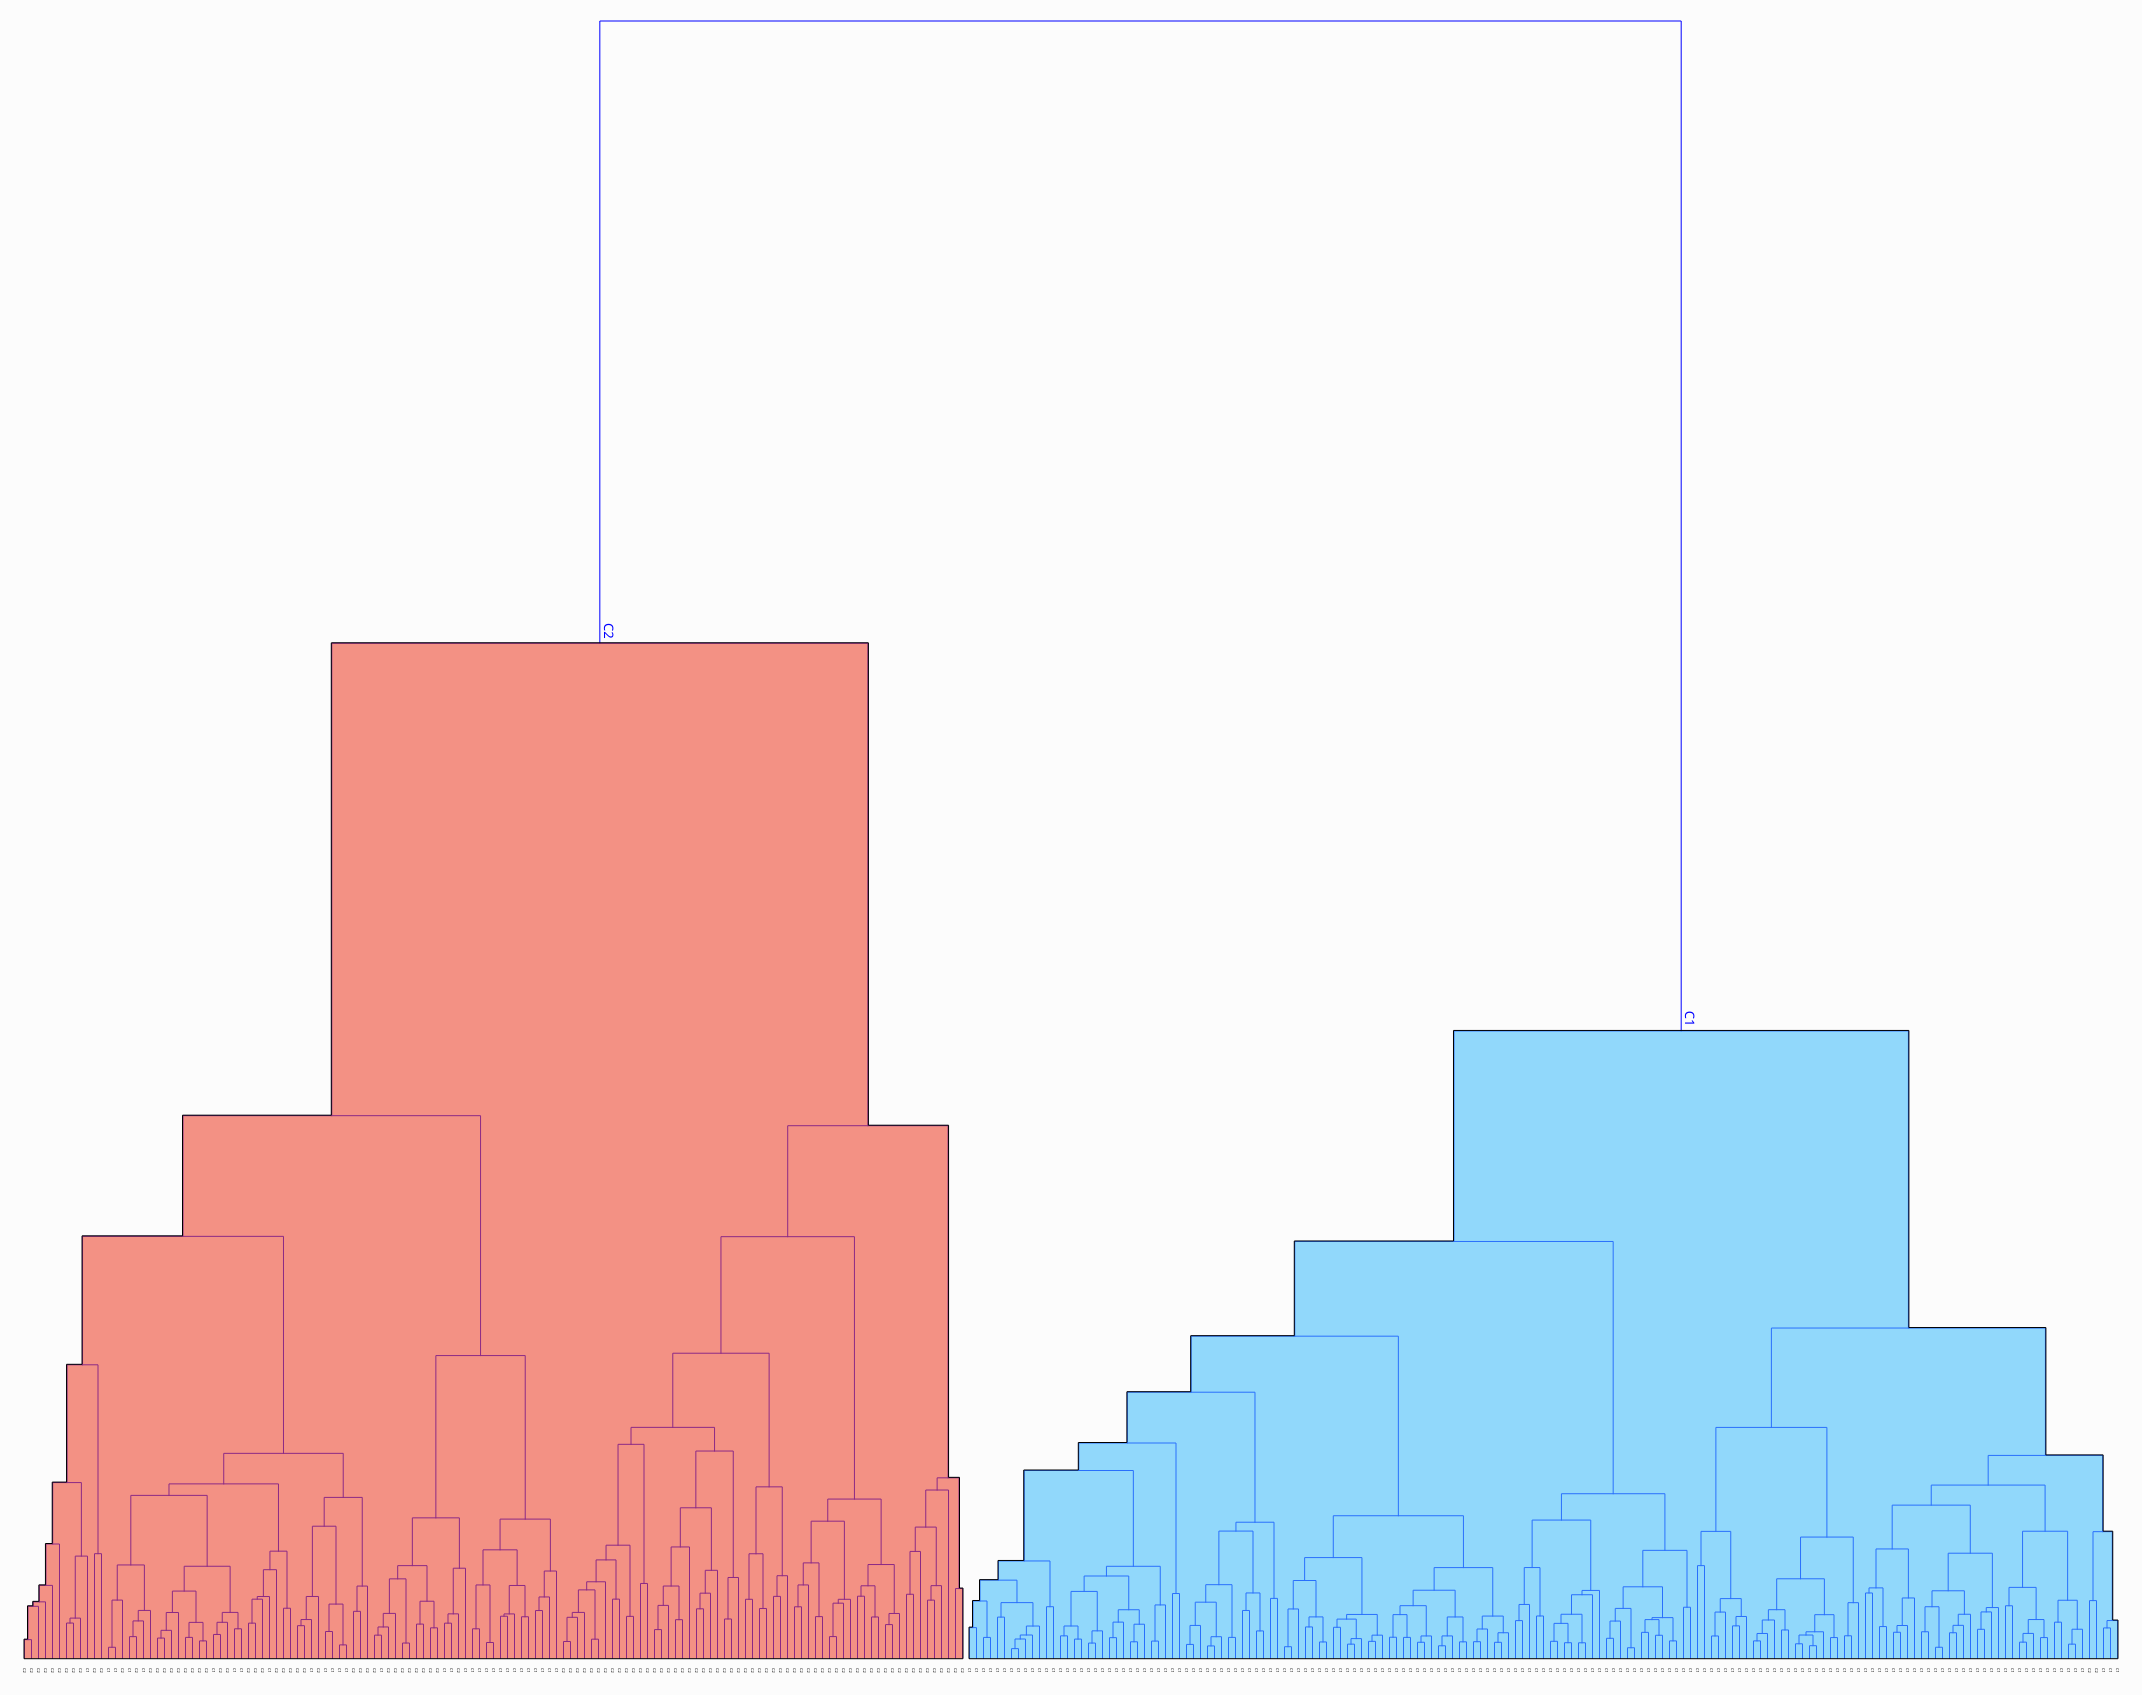
\includegraphics[width=8.1cm]{hierarchical.png}
    \caption{Hierarchical clustering}
    \label{fig:hierarchical}
\end{figure}

\subsection*{Dentition dataset}

The dentition dataset is a collection of data on the tooth pattern of 66 different mammal species. The attributes include the name of the animal, number of top incisors, bottom incisors, top canines, bottom canines, top premolars, bottom premolars, top molars, and bottom molars.

In order to find a good number of clusters to represent the data,  the same approach presented in the previous section was employed: the k-Means algorithm was used to find k clusters with k ranging from 2 to 8. An analysis of the Silhouette Score of each run indicated that 8 clusters offered a better separability of data and, therefore, more information gain.

\begin{figure}[htbp]
    \centering
    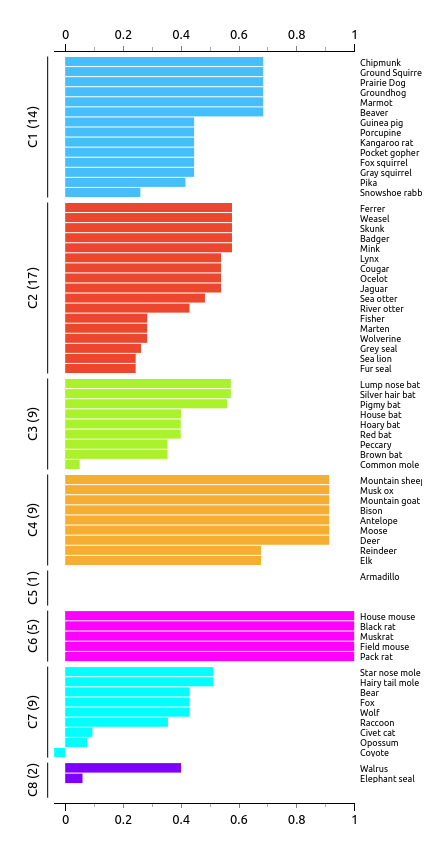
\includegraphics[scale=0.5]{k8.png}
    \caption{Silhouette plot of hierarchical clustering for 8 clusters}
    \label{fig:sil_8k}
\end{figure}

The experiment was repeated for $k = 3$ to compare the results with different linkage criteria, which determines the distance between clusters as a function of the pairwise distances between data.

Single linkage, Figure \ref{fig:single_linkage}, is the measure of the distance between the two closest points of each cluster. Although the algorithm was run to find 3 clusters it is easy to see that there is not much information gain since both C1 and C2 clusters are very small compared to C3. Cluster 2 has arguably some semantic sense to it since the animals seem to be similar to one another, but Cluster 1 has only one class and the remaining Cluster is simply composed by the rest of the data.

\begin{figure}[htbp]
    \centering
    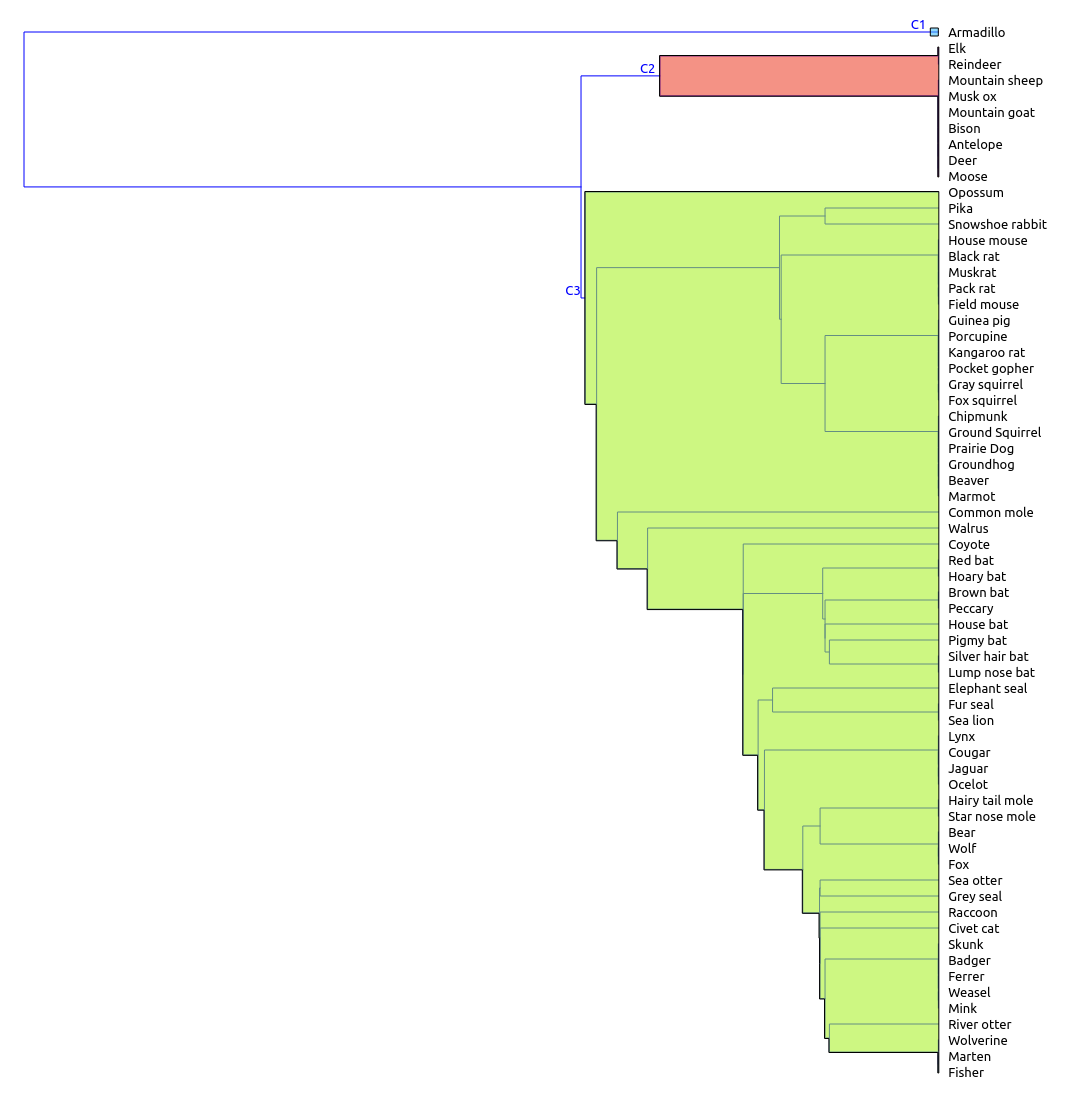
\includegraphics[scale=0.2]{single.png}
    \caption{Hierarchical clustering with single linkage}
    \label{fig:single_linkage}
\end{figure}

Average linkage, shown in Figure \ref{fig:average_linkage}, measures the average distance between every pair of points belonging to different clusters. With this approach, Cluster 2 seems to have incorporated small animals as well. In spite of C1 being still composed by a single sample, the result of this clustering approach offers much more separability of data compared to the previous approach.

\begin{figure}[htbp]
    \centering
    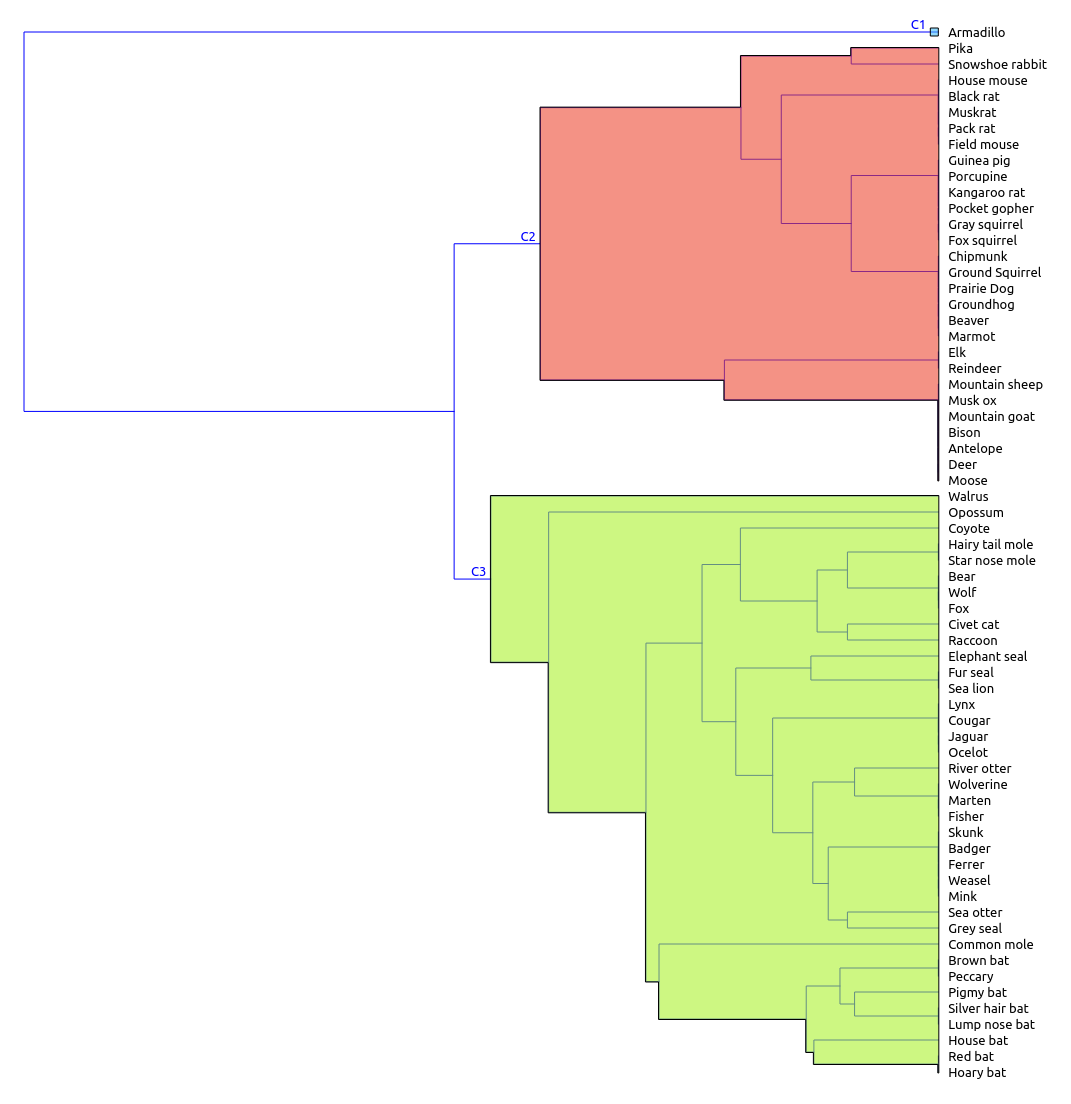
\includegraphics[scale=0.2]{average.png}
    \caption{Hierarchical clustering with average linkage}
    \label{fig:average_linkage}
\end{figure}

\clearpage

Complete linkage is similar to the single linkage, but it measures the distance between the two points that are the farthest away of each other. Again, C1 is very poor in information and only represents a single instance of the dataset, but in this experiment, C3 is very clearly formed by two well-separated inner clusters. This indicates that the same experiment for 4 clusters could produce a richer output, with 3 well-defined clusters and a cluster formed by what seems to be an outlier.

\begin{figure}[htbp]
    \centering
    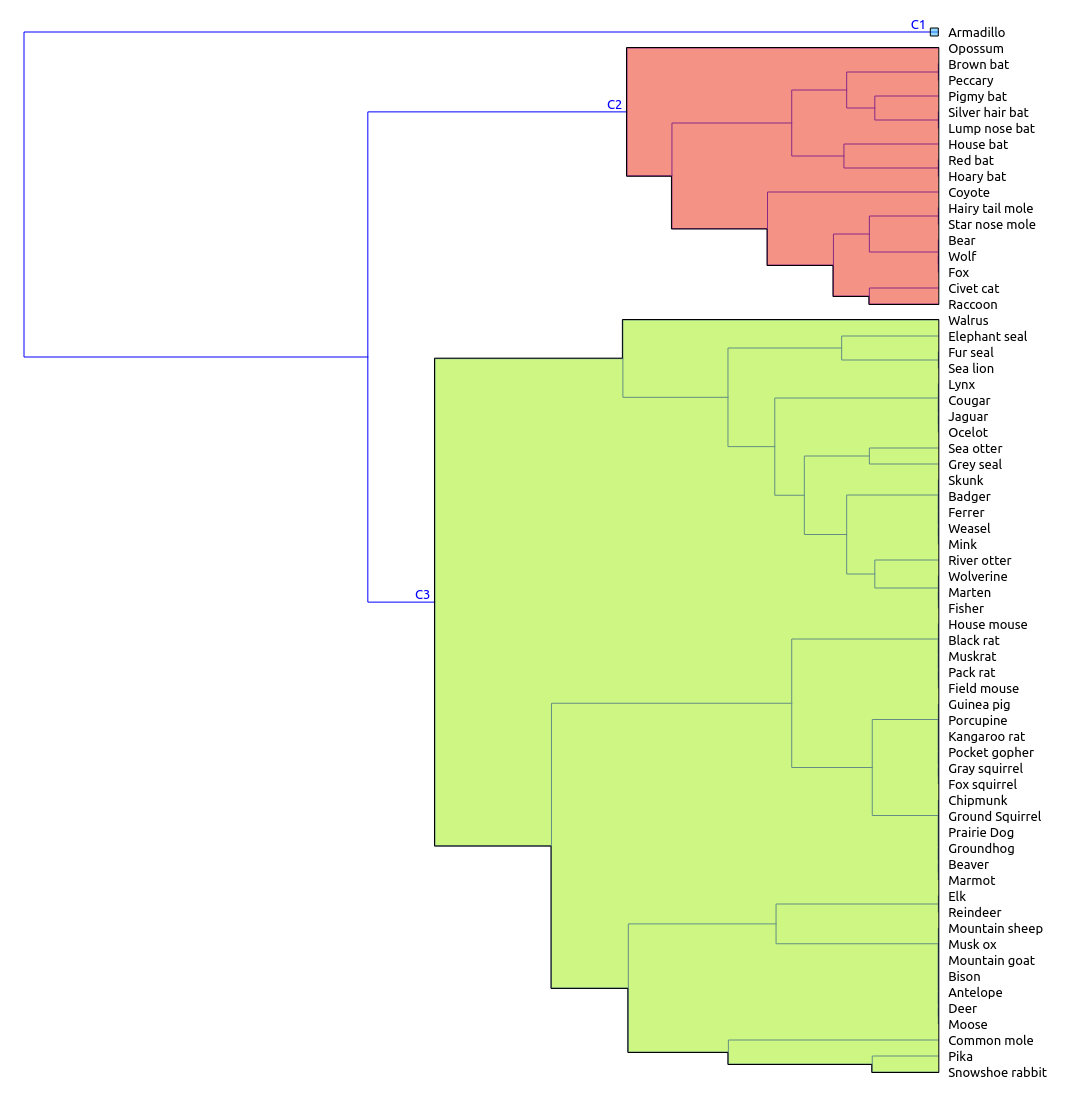
\includegraphics[scale=0.2]{complete.png}
    \caption{Hierarchical clustering with complete linkage}
    \label{fig:complete_linkage}
\end{figure}

Ward linkage was the last experiment performed on this dataset and the results show that it was the only linkage method used to generate 3 well-defined clusters. Once again, the larger cluster (C1) seems to be made of two smaller inner clusters that could provide an even better separation of data.

\begin{figure}[htbp]
    \centering
    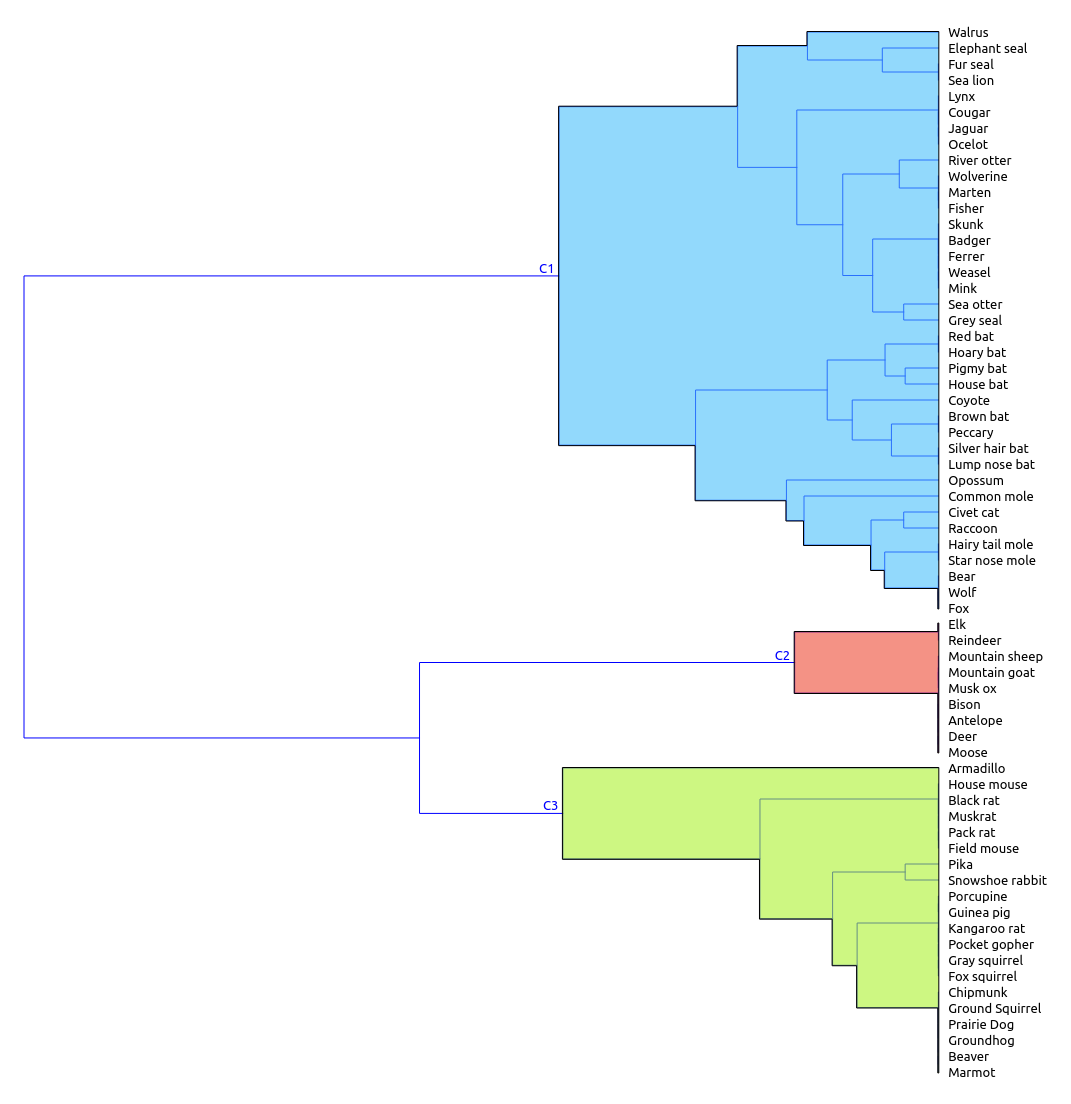
\includegraphics[scale=0.2]{ward.png}
    \caption{Hierarchical clustering with ward linkage}
    \label{fig:ward_linkage}
\end{figure}


\end{document}
 \documentclass{article}

